%% This document gives an example on how to use the gucmasterthesis
%% LaTeX document class.

%% Use short name MMT MIS or CIMET, and language,  english or norwegian
\documentclass[MACS,english]{gucthesis}

\usepackage[T1]{fontenc}
\usepackage[utf8]{inputenc}     % For utf8 encoded .tex files allows norwegian characters in the files. This can be dangerous if you change to a differnt editor.
\usepackage[pdftex]{graphicx, hyperref}   % For cross references in pdf
\usepackage{color}              % For colouring text   
\usepackage{url}

\begin{document}

\thesistitle{Investigating the Use of Context History in Task Management}
\thesisauthor{Lars Erik Strand}
\thesissupervisor{Rune Hjeldsvold}
\thesissupervisorA{Mariusz Nowostawski}
\thesisHostInstitution{\GUC}

\gmtkeywords{Context-history, Task Management, Todo-list}
\gmtdesc{This is the short description of a masters thesis}

\thesisdate{\gucthesisdate}
\useyear{03.11.2014}


 % this is the file which contains all the details about your thesis
\makefrontpages % make the frontpages
\thesistitlepage % make the ordinary titlepage

\chapter*{Abstract}

Some abstract \ldots

%\include{summary}

\chapter*{Preface}

I would like to thank \ldots Also, a special thanks to \ldots




\tableofcontents

% Comment with a percent to remove figures or tables:
\listoffigures
\listoftables


\chapter{Introduction}
\label{chap:introduction}



\section{Topic}
Task and time management applications help users stay organized by keeping track of notes, meetings, tasks etc. Many applications exist that are directed towards this purpose, ranging from simple note-taking applications and to-do lists to more advanced ones like calendars and scheduling applications. A calendar typically holds events or appointments for a user while a to-do list will keep more detailed and lower level tasks. All of these applications have in common that they relieve the user of having to remember things, thus allowing the user to focus more deeply on other things.

Context awareness is also a field of research that has received more attention in recent years. The reason for this is the increasing number of mobile devices that are available and also the increasing functionality of these devices. When it comes to context awareness, the sensors in mobile devices play a huge role. There are more sensors packed into these devices now than ever before, which allows applications to collect very specific types of contextual information. This in turn allows for the development of applications that have very specific and tailored purposes.

By combining context awareness and task management, we open up for new types of applications. Smarter systems could be built that leverage contextual information, both past and present, to adapt its behavior to accommodate very specific situations. A calendar system for example, could evaluate a user's upcoming meeting and the current location of the user. Taking into account the distance between the user and meeting location, the system could then deliver a reminder at the appropriate time, allowing the user to catch the meeting. Another example would be a to-do list application that could leverage contextual information about previously performed tasks to provide task recommendations to the user.





\section{Problem description}
Task and time management applications are valuable tools that are used by many people. These applications can be especially valuable on mobile devices as the users can carry these devices with them, thus having the application data easily accessible. Concrete and popular examples of such applications are calendars such as Google Calendar\cite{googlecalendar} or to-do list applications such as Trello\cite{trello} or Todoist\cite{todoist}. Even though these, and many similar applications are very useful, their functionality and usefulness could be further improved by integrating user context. 

Utilization of contextual information in different scenarios have been widely researched. However, we have found no research that studies the usage of such information in the specific domain of task and time management systems. Many systems are improved by making them context-aware. One example of this is Learning Management Systems (LMS) that can suggest learning content based on the users current context\cite{verbert2012context}, and in doing so increasing the level of learning for the user. Following examples such as this, it is believed that task management applications can also reap the benefits of context awareness.

This study will look into the area of utilizing contextual information in task management applications. We will design a proof of concept application that tries to make use of the user's contexts.

\section{Justification, motivation and benefits}
The complete envisioned application is a personal information manager (PIM) where the user only needs to inform the application of the tasks that he/she needs to perform. The application would then suggest a current task and provide an optimal ordering of the other tasks, taking into account the current user context. This optimization can for example be based on minimizing total time spent completing the tasks, minimizing total travel distance between tasks, thereby reducing travel costs and pollution, or a combination of these. With respect to time, this would mean that completing the tasks in any other order than that suggested by the system would lead to a longer time spenditure. In order to create such a system, many areas would need extensive research, more than that which is possible to complete within the scope of this thesis. However, sub-parts of the system can be identified and researched, providing building blocks for the realization of the entire system. These sub-parts include how to collect relevant context data, how to store those data, how to implement an overall design of such an application and how to evaluate past tasks and contexts to successfully produce task suggestions. Identifying and researching these parts of the system justifies the work to be conducted in this thesis, as it allows for working towards the higher-end goal. The motivation behind the thesis is to be able to contribute to to-do applications, and by extension task management applications in general, by further enhancing their task management capabilities.



\section{Research questions}

This thesis is three folded. Firstly, there is the area of context collection and representation. Secondly, we have the software engineering area, which relates to application design and functionality. The third area revolves around the context in which the previous two are placed for this thesis, namely students and the educational context for which the thesis is conducted in. The proposed solution will have to address all of these areas in detail. Therefore, these research questions have been formed for each of the areas:
\begin{itemize}
	\item \textbf{Research question 1}: What contexts are relevant in a task management application, and how can they be acquired and modeled?
	\item \textbf{Research question 2}: How can a task management application be designed and what are the important design decisions when making such an application?
	\item \textbf{Research question 3}: How can context information be utilized in a task management application?
\end{itemize}

\section{Thesis structure}
Chapter~\ref{chap:relatedwork} provides the necessary background that related to the work in this thesis. State-of-the-art task management applications are also covered here. Chapter~\ref{chap:methodology} describes the whole process of designing the to-do list application and is also in its entirety the answer to research question 2 and 3. Chapter~\ref{chap:results} presents the findings in this thesis and is together with Chapter \ref{chap:methodology} and \ref{chap:discussion} the answer to research question 1. Chapter~\ref{chap:discussion} discusses the different approaches and decisions made in this thesis, as well as discussing alternatives for some of these decisions. The work is then concluded in Chapter~\ref{chap:conclusion} and futer work is discussed in Chapter~\ref{chap:futurework}.
\chapter{Related Work}
\label{chap:relatedwork}



\section{Context awareness}

Context awareness is a large area of research. This has led to many proposed definitions of context and context awareness \cite{liu2011survey}. Context can refer to many different things, in fact, everything that happens in everyday life, happens in a context. Because of this, it is important to provide a specific definition of context when researching the area in order to avoid confusion. This thesis will use a widely used and commonly accepted definition of context proposed by Dey \cite{dey2000providing}, stating that:
\begin{quote}
``Context is any information that can be used to characterize the situ-
ation of an entity. An entity is a person, place, or object that is considered
relevant to the interaction between a user and an application, including the
user and application themselves.''
\end{quote}
Following this, a context-aware application is therefore an application that gathers contexts, interprets them, and adapts its behavior accordingly during runtime to adjust to the users situations and needs.


\section{Collecting contexts}

In a mobile device there are typically many types of contexts that can be  collected via the system and its sensors. Some of these are:
\begin{itemize}
	\item Location
	\item Movement
	\item Time
	\item Activity
	\item Air pressure
	\item Ambient sound
	\item Humidity
	\item Orientation of device
\end{itemize}


\section{Context history}

Context-history refers to persistent storing of contextual information, in order to use this information for future purposes. The limitation of current to-do list applications is that they do not propose the usage of context-based history, and only considers current context. Utlilizing context-history usually involves reqognizing patterns in the stored context information. Studies involving context histories is also limited in the sence that most of them focus on building histories rather than utilizing them \cite{chalmers2004historical}.

A study looking into the utilization of context-histories has been presented in \cite{hong2009context}. This study tries to predict the preferences of the user by utilizing context-history. They implement a context management layer into their system where an inference agent infers the high level contexts from the raw, sensed contexts. These high level contexts are then stored as context-history represented by the OWL ontology language.

One way to extract usefull information through context histories would be deducting user habits from them. Ciaramella did such a study \cite{ciaramella2010using}. The study proposed a resource recommender that adapts to the habits of a specific user. This adaption was based on genetic algorithms (GA's). By tracking user behavior on a mobile device, they collected the context-history and utilized fuzzy linguistic variables to handle vagueness in the collected data. The study showed that adding context-histories and GA's to the calculation of recommended resources, improved both responsiveness and modeling capabilities of the recommender.



\section{Making predictions based on context}

Mayrhofer et al. discuss some issues regarding context-prediction \cite{mayrhofer2005context}. When trying to predict a user context in order to proac1tively perform a task for the user, it is important that the predictions are accurate. This is generally a significant problem in the area of context prediction. This thesis is not focused on proactively performing tasks for the users. It is focused on providing task suggestions based on these predictions, thereby making the problem slightly less significant. However, the user experience will be related to the accuracy of these suggestions, meaning that it will still be of some importance.

When making predictions based on contexts, how the prediction is performed is equally important as that which is predicted. A study on how to proactively determine spatial data about the user is done in \cite{anagnostopoulos2005prediction}. Here, a Predictive Context Object (PCO), modelled in UML, is proposed for modelling predictive data. A prediction algorithm is also proposed, consisting of concrete mathematical formulae.



\section{Context abstraction and modeling}

Many studies have looking into context modeling and representation \emph{\color{red}(reference(s) here)}. Context modeling and representation studies is often about providing proper abstraction from the raw context data. However, by using the integrated features for collecting contexts in Android, such abstractions are already built into the framework. Instead of getting raw contextual data from the framework, we can get data that are ready to be used and stored directly. For location contexts for example, we could get GPS coordinates, or even a specific address. For a user activity context we could get the data as a string indicating whether the user is \emph{still}, \emph{on foot} or \emph{in vehicle} to name a few. 

\section{Intelligent task and time management systems}
The SELF-PLANNER \cite{refanidis2011deployment} proposed an intelligent Web-based calendar system where a users schedule can be created automatically by the system \cite{refanidis2010constraint}. Research in intelligently scheduling a user's activities also touches the field of Artificial Intelligence (AI). The study investigates different types of user activities, such as activities that are dependent upon each other, interuptable activities, location-dependent activities, and activities of variable length. It also studies how these activities can relate to each other in order to create a model of the activities to be used in the scheduling algorithm. The work was based on the Squeaky Wheel Optimization framework, and shows that letting an intelligent system schedule user activities can generate effective and qualitative plans \cite{refanidis2010constraint}.

Norton et al. proposed a information management system that can autonomously rearrange a task list depending on the current user context \cite{norton2010towards}. The system is similiar to a to-do list application. The paper studies relationships between tasks based on their priorities, deadlines, and locations in order to autonomously rearrange tasks with respect to time optimization. However, the system does not suggest using context history for this purpose. The paper also focus more on a smart way to recieve location data in order to save battery power. Trending (history) is mentioned, but this is purely for location and to further optimize the battery life. For ordering the tasks the system normalizes the relevant factors and use a multi-dimensional Euclidean space to determine the ordering.

Research presenting automated task assistants have also been proposed. Towel \cite{conley2007towel} propose a intelligent to-do list system, allowing for simple user task to be automatically performed by a system agent. The users to-dos are integrated with the execution-agent, called Project Execution Assistant (PExA) \cite{myers2005cognitive}. The tasks that the agent can perform need to be rather simple tasks that the agen can interpret and fully comprehend in order to do the tasks correctly. Such tasks include sending emails, looking for available hotels and arranging meetings. By relieving the user of these trivial tasks, the user can then focus on more important task requiring human problem solving skills.

A similar study was presented in \cite{myers2007intelligent}. This study proposed a system architecture for task and time management systems. This system's purpose is also to relieve a user from routine tasks, so that the user can focus on more complex tasks, thus increasing productivity among knowledge workers. The utilization of PExA are more thoroughly described in this study. A possible shortcoming in the study is that the agent performing the user tasks, need to be given specific instructions on a high level of detail by the user. This means that a method for infering data about a user task is not proposed.

Driver and Clarke proposed something that they called context-aware trails \cite{driver2008application}, which is a list of scheduled activities. Activity scheduling based on context can help users in many different areas, such as a hospital worker needing to do patient rounds and administrative tasks. Generating these trails has some problem areas that are much like the Traveling Salesman Problem (TSP) \cite{lawler1985traveling}. The mechanism for generating the trails is based on context-based activity set reduction, where the activity set is the entire list of activities the user could do while using the application.

The reviewed proposals are relevant for task and time management systems. However, none of these systems have looked into the use of context-histories for their purposes.




\subsection{Alternative recommendation algorithms}
Neural networks describes the process in which the computer\ldots
(half a page with a couple of references\ldots)

\subsection{Probability calculations}
The second approach is to use probability calculations to perform the recommendations. This is the approach that was decided to be used in this project. \emph{\color{red}(some general information + a couple of references\ldots)}

\chapter{Methodology}
\label{chap:methodology}

In order to address the research questions, we need to develop a proof of concept system that is able to investigate and utilize the concepts in question. It was decided that a to-do list application would be a good candidate for investigating these concepts. A to-do list application is a task management system in a simple form. The simplest version of it could be just a list of strings representing the user's tasks, or to-do items, that needs to be done. Another form of a task management system is a calendar. A calendar would also be a suitable candidate for looking into the use of contexts in task management. However, a calendar is more complex than a to-do list, even in its simplest form, and would require more design decisions than a to-do list if building a system from scratch. Considering this, a to-do list application was chosen.

When building context-aware systems, the most natural choice of platform is mobile devices. Contextual information is readily available on such devices because of their cheap and integrated sensors, which now exists on nearly all modern handheld devices. It is easy to access information such as user activity, time and location. The two most popular operating systems for such devices are Android and iOS. The development frameworks for both of these have functionality that allows for easy acquirement of context data. Even context abstraction and representation are handled by the frameworks, so that the developer no longer has to deal with the raw sensory data coming from the hardware. For this particular thesis, the Android Operating System was chosen for development. This is mostly because it holds the biggest market share by far, but also because an Android device was easily available for development.




\section{User group}
For the recommender to be able to differ between user tasks, these tasks needs to be assigned different types and be categorized. However, categorizing typical and everyday tasks will require a lot of effort. It is known that modeling an individual's tasks and activities can be challenging \cite{refanidis2010constraint}. Consider trying to generalize the tasks of an office worker and a carpenter. The tasks that these two typically do during a day, will vary greatly. Finding similarities among these tasks so that they could be generalized to fit a general population would be difficult. Therefore, in order to reduce complexity and the amount of work needed, it was decided that the scope should be narrowed down by selecting a specific user group. This will also allow for narrowing down the application itself, both in terms of general application design as well as the complexity of context collection and representation.

The user group that was selected was students, and more specifically students in an educational environment. There were two main reasons for this. One being that the tasks of such a narrowed down and specific user group can be much easier divided into separate types and categorized. We will then be able to predefine a set of tasks that should cover most of the different types of tasks that a student will be doing in an educational environment. The second reason for choosing students was that this user group was easily accessible for questioning or experimenting.

Although students were selected as the target user group, typical educational tasks can still vary to a large degree between undergraduate and postgraduate students. This can also be highly dependent on what semester the student in question is currently in. A bachelor student might have very different tasks than a master student doing his/hers master thesis. To determine these differences, and to find out whether or not eventual differences needed to be accounted for in the application design, a short questionnaire was made. Detailed results of the questionnaire can be found in Section~\ref{subsec:studenttasks}. Through the questionnaire, we found that there were only minor differences between the tasks of the different types of students. It was therefore decided that the tasks should be categorized equally for all students.

The actual task categories used for the tasks in the application were:
\begin{itemize}
	\item Attend lecture
	\item Read
	\item Write report
	\item Do course exercises
	\item Meeting
	\item Group work
	\item Practical work
	\item Other
\end{itemize}
These categories are based on the results of the short student task questionnaire we made. We provided a set of predefined tasks where the student had to answer how often they typically performed each task, both in terms of regularity (once a day, once a week etc.) and frequency (1-3 times a week, 4-6 times a week etc.). They students were also able to fill in additional tasks, if the predefined tasks were not enough to cover all the tasks that they typically do.



\section{Application}

\subsection{General application design}
By choosing to create a todo-list application, the user should be able to perform actions that are normal for such applications. These actions include creating and storing tasks, as well editing and deleting them. The tasks should also be possible to arrange into lists. By studying other to-do list applications \cite{trello, todoist} we came up with a set of minimum requirements that the application would have to fulfill.
\begin{itemize}
	\item Creating tasks.
	\item Editing/deleting tasks.
	\item Creating lists for tasks.
	\item Managing lists by editing/deleting them, or moving tasks between lists.
\end{itemize}
These are core features that are supported in popular to-do lists, and the users would expect a to-do list to have this functionality. The application in this study is developed in a way that supports all these aspects. When a todo-item or task is created, a date will be attached to that particular task, thereby organizing the tasks with similar dates into lists.

We want to utilize context features in our application in order to make task recommendations for the user. Therefore, we would have a few more requirements in addition to the ones mentioned above:
\begin{itemize}
	\item Collection of contexts
	\item Modeling and representing the contexts in a way that it can be utilized.
	\item A recommender module to process the tasks and contextual information.
\end{itemize}

With the above requirements in mind, we designed a conceptual model of the application, shown in Figure~\ref{fig:conceptualmodel}.
\begin{figure}[tbp]
  \centering
  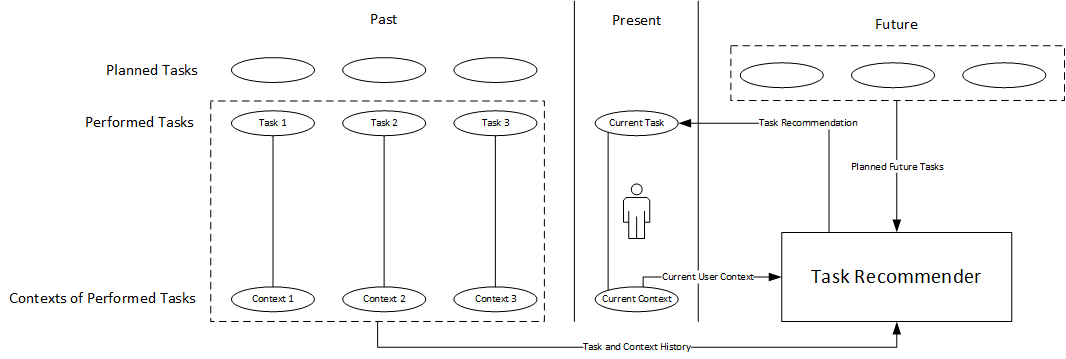
\includegraphics[width=\textwidth]{figures/ConceptualDiagram.png}
  \caption[Conceptual model]{Conceptual model of the application.}
  \label{fig:conceptualmodel}
\end{figure}
The figure shows the general idea behind the application. We have the user in the center in the current context. To the right we have all the tasks that the user has planned in the application. When these tasks are being done the contexts of the user are tracked, and upon completion stored together with the tasks in the database, as shown on the left. Here, the completed tasks and their related contexts make up the task and context history.

The recommender is a separate and independent module in the application. The lines pointing towards the recommender represents its input, whereas the line pointing outward is the output, i.e. the actual task recommendation. The input for the recommender consists of three parts:
\begin{itemize}
	\item The tasks that the user needs to do (planned tasks).
	\item The tasks that the user has previously done (task history) and the contexts related to these tasks (context history).
	\item The users current context.
\end{itemize}
By taking all these components into account, the recommender will be able process the information and suggest a task for the user. The recommender is discussed more thoroughly in Section~\ref{sec:recommender}.

In the overall design of the application, we decided to stay with the Android design principles\cite{androiddesign} as much as possible. Popular apps on Google Play tend to follow similar design patterns, which means that Android OS users are accustomed to a certain look and feel. We wanted to provide a look and feel in our application that would be familiar to the users, in this case the students using the application. The graphical design of the main application screen is shown in Figure~\ref{fig:designmainscreen}.
\begin{figure}[tbp]
  \centering
  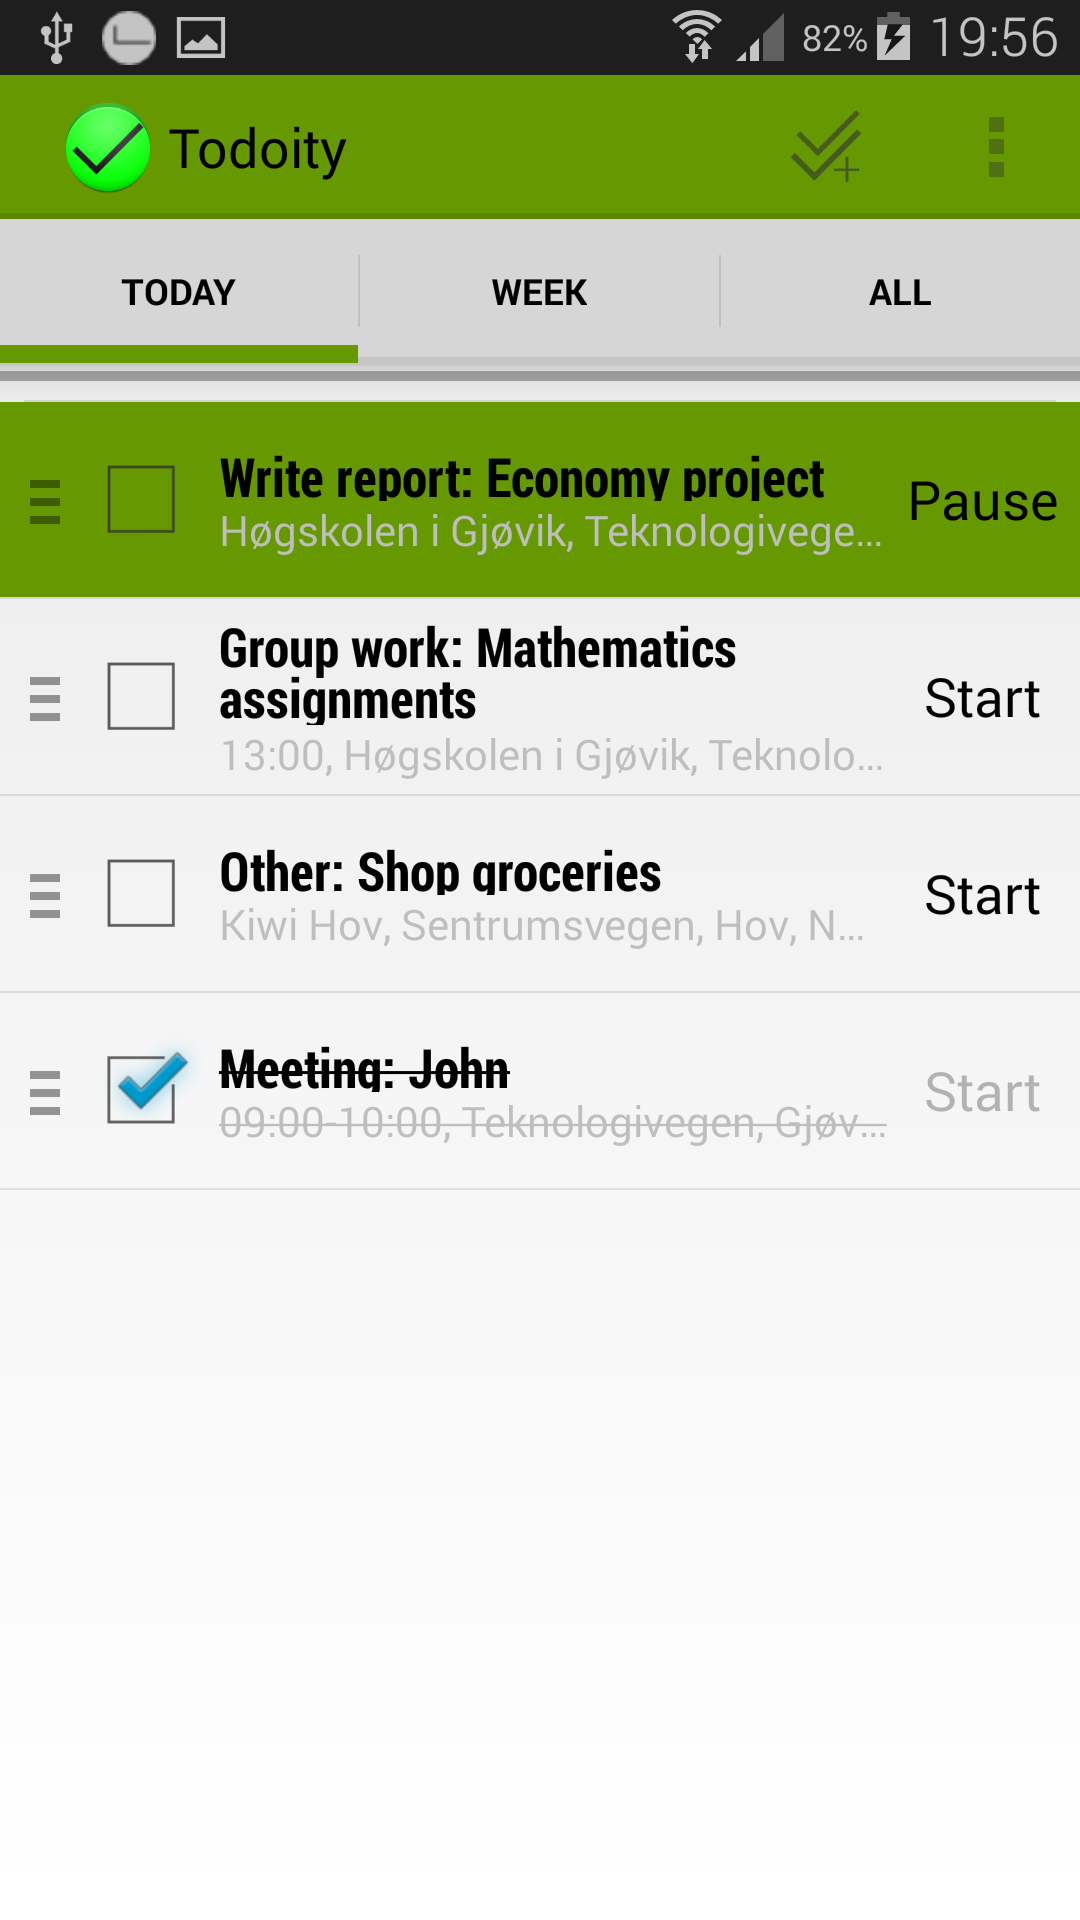
\includegraphics[width=0.35\textwidth]{figures/MainScreenStarted.png}
  \caption[Main application screen]{The main screen of the application, showing a few tasks where one is ongoing and one is finished.}
  \label{fig:designmainscreen}
\end{figure}
Here we can see several similarities with the design guidelines. There is a toolbar with common actions at the top (new task button and an overflow menu with settings and about) which is also given a app-specific color that runs through several other parts of the application (also called branding). We also provided tabs to allow the users to easily change between viewing both future planned tasks and past tasks. The \emph{today} tab is the default tab, displaying the tasks that the user has planned for the current day. Tasks that have been started by the user is placed at the top of the list and given a background color to indicate that it is running. Finished tasks are automatically placed at the bottom. The user also have the option to reorder the tasks through drag and drop.

A slightly simplified version of the overall workflow of the application is shown in Figure~\ref{fig:workflow}.
\begin{figure}[tbp]
  \centering
  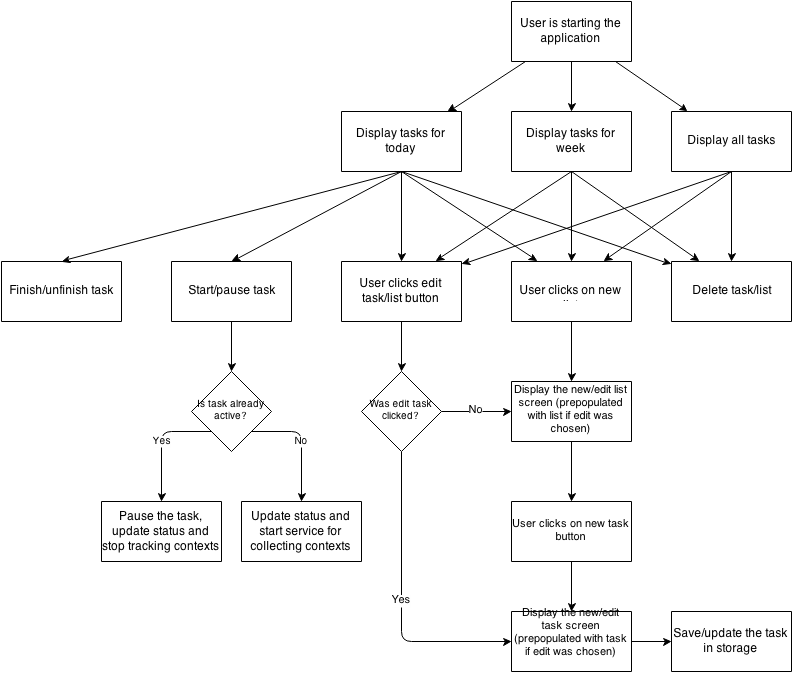
\includegraphics[width=0.7\textwidth]{figures/Workflow.png}
  \caption[Application workflow]{Application workflow.}
  \label{fig:workflow}
\end{figure}
This depicts the basic functionality that is provided. 

When the users launches the application, the \emph{today} screen is shown by default. From here, the user can create a new list of tasks, add tasks to current lists or delete tasks or lists. Upon selecting a list, the user can edit and delete existing tasks within that list or create new tasks. When wanting to edit or create a new task the user is directed to the new task screen. This is where the actual information about the task is entered. The creation of a new task is shown in Figure~\ref{fig:newtask}.
\begin{figure}[tbp]
  \centering
  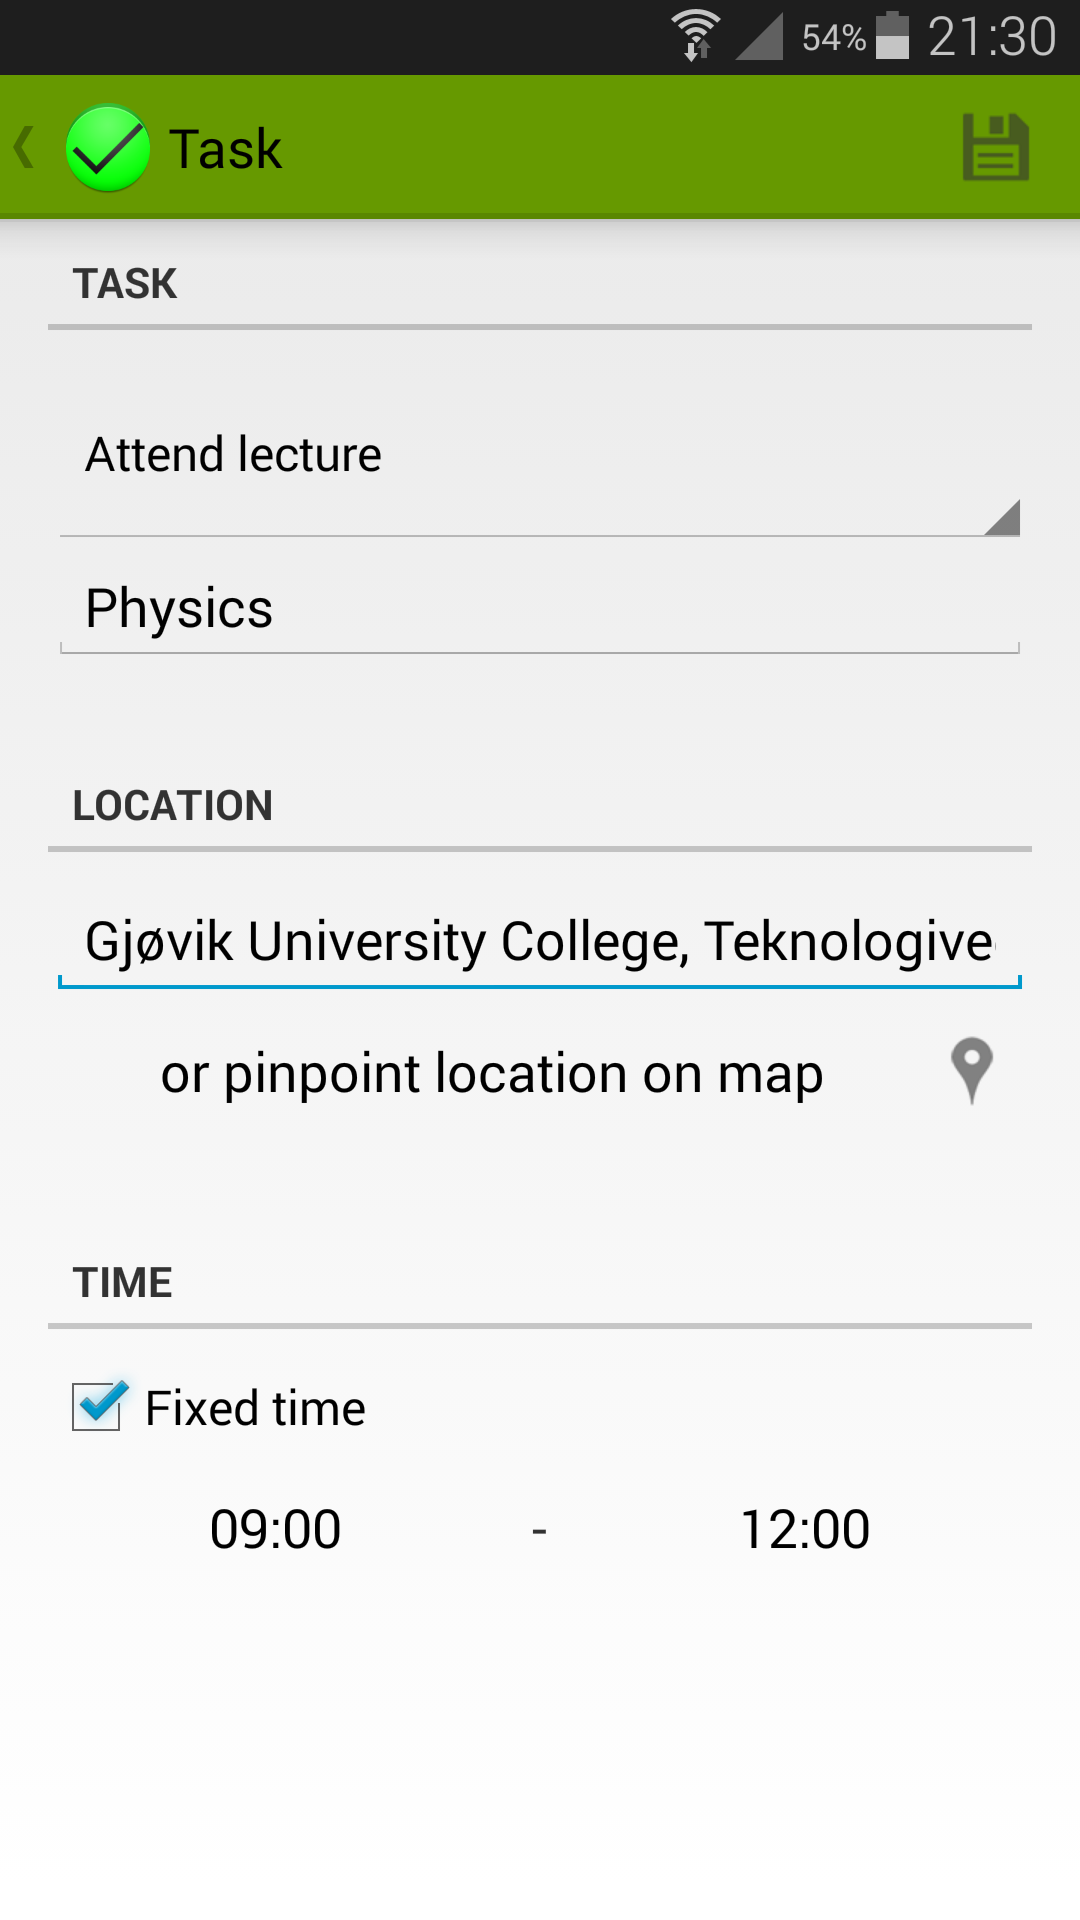
\includegraphics[width=0.35\textwidth]{figures/NewTask.png}
  \caption[Screen for creating a new task]{Creating a new task.}
  \label{fig:newtask}
\end{figure}
A category for the task has to be entered here. This is done by selecting one of our predefined tasks from a list. The user can also provide an optional description for the task. For this thesis, it was decided that a location should also be required by the users to provide. This is because we are designing a context-aware application that heavily relies on location. However, for a commercialized version of the application, a location would probably not be required as the users might get tired of having to input a location for every task. The location can either be input as text, where an autocomplete function was implemented to help users select real locations, or the map button can be clicked, which lets the user pinpoint the location from a map. The tasks can also have a fixed starting time and/or end time, which is optional.

\subsection{Context acquisition}
By storing contextual information about how tasks are performed, the recommender will be able to not only provide recommendations based on current and planned contexts, but also take into account in what contexts tasks have been done previously. A certain task may work well in one context and poorly in another. However, before designing the overall schema of context representation, decisions on what contexts to actually use and collect needs to be made. In a mobile device there are typically many types of contexts that can be  collected via the system and its sensors. Some of these are:
\begin{itemize}
	\item Location
	\item Movement
	\item Time
	\item Activity
	\item Air pressure
	\item Ambient sound
	\item Humidity
	\item Orientation of device
\end{itemize}

Although all of these contexts, and more, could be collected by a mobile device, not all of them would be equally relevant to use in a to-do list application. While each of the contexts could be used to some degree, there are situations were some contexts would be redundant. Humidity, for example, could be a somewhat useful context for someone working on very specific tasks in very specific environments, say an environmentalist taking water samples near lakes and rivers. However, for students in an educational environment, such contexts are less relevant.

The actual contexts that was decided to be collected in the app were:
\begin{itemize}
	\item \emph{Location:} Both the planned location of the task as well as the actual location of where the task is performed is stored.
	\item \emph{Activity:} The movement of the device while contexts are collected.
	\item \emph{Time:} Each task is given timestamps both when they are started and ended. By doing this it is possible for the recommender to separate tasks that are done at specific times of the day, week or even month. Time spent doing a task is also tracked, as this may differ from the difference between the start and end times (users may pause doing a task).
\end{itemize}

The actual logic behind the tracking of tasks and their contexts is a separate problem. It was decided that the tracking if tasks would have to be manually started and stopped by the users. This was done by providing a start button for each task, as shown in Figure~\ref{fig:taskrepresentation}.
\begin{figure}[tbp]
  \centering
  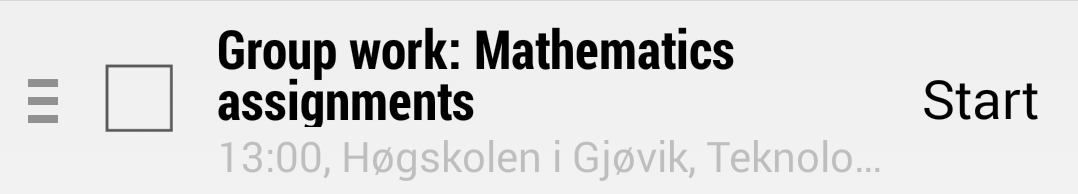
\includegraphics[width=0.5\textwidth]{figures/TaskRepresentation.png}
  \caption[In-app representation of task]{The in-app representation of a planned task.}
  \label{fig:taskrepresentation}
\end{figure}

\section{Context storage and modeling}
A database was needed to store both the collected contexts and the tasks. Both an internal and external database was chosen to hold the data. An internal database was chosen because it is easy to implement as well as it allows for the application to be used while being offline. However, in order to easily retrieve and analyze the collected tasks and contexts for the thesis results, an external database was chosen. While the internal database only holds information regarding the specific installation, the external database holds all the information about all installations, i.e. all tasks and all contexts from all users. We used the Android built-in SQLite database for the internal storage and Google's AppEngine datastore for the remote storage.

While many studies have looking into context modeling and representation \emph{\color{red}(reference(s) here)}, we decided to go with a normalized database approach. Context modeling and representation studies is often about providing proper abstraction from the raw context data. However, by using the integrated features for collecting contexts in Android, such abstractions are already built into the framework. Instead of getting raw contextual data from the framework, we can get data that are ready to be used and stored directly. For location contexts for example, we could get GPS coordinates, or even a specific address. For a user activity context we could get the data as a string indicating whether the user is \emph{still}, \emph{on foot} or \emph{in vehicle} to name a few. The representation of the data for the application is shown in Figure~\ref{fig:databasemodel} and Figure~\ref{fig:databasemodelexternal}
\begin{figure}[tbp]
  \centering
  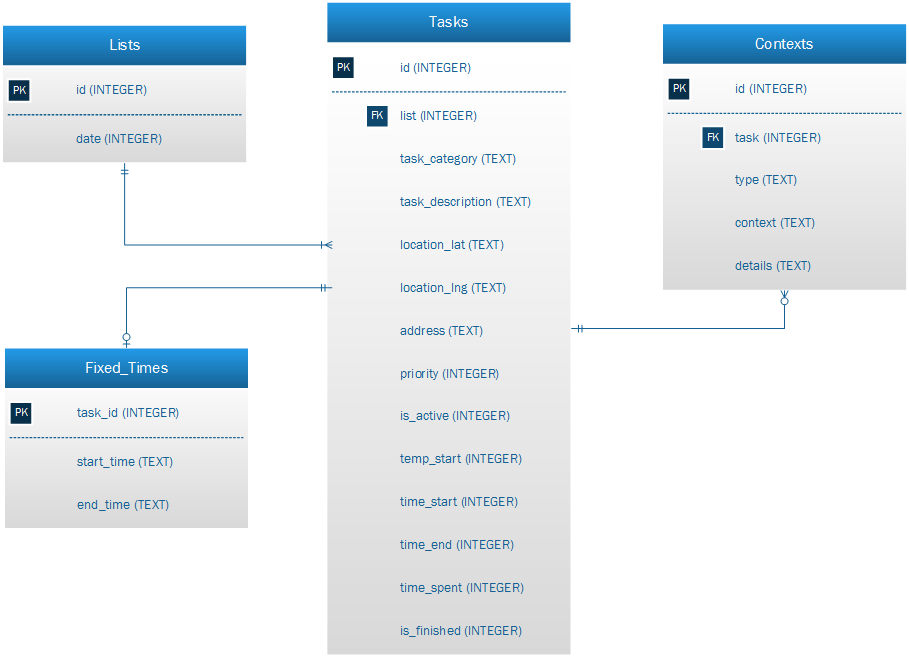
\includegraphics[width=0.8\textwidth]{figures/DatabaseModel.png}
  \caption[Database model]{SQLite representation of the individual installations application data.}
  \label{fig:databasemodel}
\end{figure}
\begin{figure}[tbp]
  \centering
  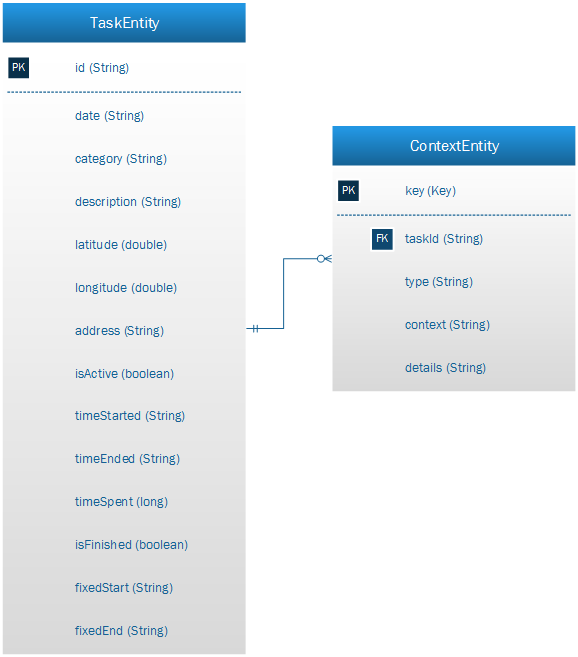
\includegraphics[width=0.5\textwidth]{figures/DatabaseModel_external.png}
  \caption[External database model]{The Google AppEngine datastore representation for all installations application data.}
  \label{fig:databasemodelexternal}
\end{figure}

The actual acquisition of the context data happens when the users starts a task from the application. A background service is then started and runs on the device until the task is paused by the user or completed. The service collects these contexts at certain intervals. If a collected context, for example location, is already collected for a specific task then that context is not stored again. Multiple identical locations for a single task is not needed, so this prevents some information overhead.




\section{Recommender}
\label{sec:recommender}

When creating the recommender part of the application, several decisions needed to be made. First of all, we needed to decide what kind of recommendations to make. There where many possible ways to do this:
\begin{itemize}
	\item Location proximity recommendations.
  \item Recommendations based on time of day.
  \item Recommendations based on time spent on previous tasks.
  \item Recommend tasks with fixed starting times.
  \item Recommend tasks based on the shortest traveling distance between tasks.
  \item Recommendations based on regularity of task occurrences.
  \item Combinations of the above.
\end{itemize}

After deciding what to recommend, the underlying logic also needed to be decided. A recommender will need some form of logic for comparison, so that it can know that it should recommend one task over another. Such logic already exist in some systems. We have seen Netflix\cite{netflix} recommend movies and Amazon\cite{amazon} recommend books to name a couple. It is potentially beneficial to analyze other systems for reusable recommendation algorithms.

\subsubsection{Neural networks}
Neural networks describes the process in which the computer\ldots
(half a page with a couple of references\ldots)

\subsubsection{Probability calculations}
The second approach is to use probability calculations to perform the recommendations. This is the approach that was decided to be used in this project. (some general information + a couple of references\ldots)

Unfinished \ldots

\subsection{Chosen recommendation algorithm}

As mentioned earlier, the input for the recommender consist of the users planned task, the current context, and the entire task history with related contexts. The recommender starts by looking at the categories of the user's planned tasks and tries to calculate a probability for each of them, representing how likely the task is going to be chosen next by the user. This calculation is done based on the tasks that the user has previously done and in what contexts. Probability calculations are made individually for each of the different contexts, but also for combinations of them. For example, the recommender will consider the current time of day and then find other tasks that have been done during the same time of day previously. The probability for a specific task is then calculated by dividing the number of occurrences of that particular task by the total number of tasks performed at that time of day. This is done for each of the tasks that the user has planned and the result is put into a map, as shown in Table~\ref{tab:probabilitymaptimeofday}.
\begin{table}[tbp]
  \centering
  \begin{tabular}{|l|r|}
	\hline
	\textbf{Task category} & \textbf{Probability} \\
	\hline
	Attend lecture & 0.11 \\
  \hline
	Other & 0.24 \\
	\hline
	Practical work & 0.46 \\
	\hline
	Read & 0.14 \\
	\hline
	Write report & 0.05 \\
	\hline
  \end{tabular}
  \caption{Example recommendation probability hashmap}
  \label{tab:probabilitymaptimeofday}
\end{table}

The same process is executed for other contexts as well. For example, based on the current location of the user, the recommender finds all tasks that have been performed in that particular location. Probabilities are then calculated the same way as for the time of day. The task probability map based on location may look like Table~\ref{probabilitymaplocation}.
\begin{table}[tbp]
  \centering
  \begin{tabular}{|l|r|}
	\hline
	\textbf{Task category} & \textbf{Probability} \\
	\hline
	Attend lecture & 0.41 \\
	\hline
	Other & 0.13 \\
	\hline
	Practical work & 0.25 \\
	\hline
	Read & 0.16 \\
	\hline
	Write report & 0.05 \\
	\hline
  \end{tabular}
  \caption{Location recommendation probability hashmap}
  \label{tab:probabilitymaplocation}
\end{table}

Similar maps are calculated for each context and all combinations of them. This means:
\begin{itemize}
	\item Time of day
	\item Day of week
	\item Location
	\item Time of day \emph{and} location
	\item Time of day \emph{and} day of week
	\item Day of week \emph{and} location
	\item Time of day \emph{and} day of week \emph{and} location
\end{itemize}
The highest probability from each of these individual probability maps are then put into a resulting map, where the highest probability in this map will be the actual task recommendation med by the recommender. Looking at Table~\ref{tab:probabilitymaptimeofday} and Table~\ref{tab:probabilitymaplocation}, the resulting map will look like Table~\ref{tab:probabilitymapresult}.
\begin{table}[tbp]
  \centering
  \begin{tabular}{|l|r|}
	\hline
	\textbf{Task category} & \textbf{Probability} \\
	\hline
	Attend lecture & 0.41 \\
	\hline
	Practical work & 0.46 \\
	\hline
  \end{tabular}
  \caption{Resulting probability hashmap upon which the actual recommendation is made}
  \label{tab:probabilitymapresult}
\end{table}
The actual recommendation made by the recommender in this example would be the task with the category ``practical work''.

\section{Application distribution and user experiments}
To test our design decision we needed users to test the application for a certain period of time. Because the application is based on task and context history, it would take some time and usage in order for history to build up. A large history of tasks and contexts is needed so that for the recommender can make reasonable recommendations. The recommendations from the recommender should increase in accuracy over time. By accuracy we mean tasks that matches the tasks that the users intend to do next. We could say that the application is ``learning'' the users behavior over time. For this experiment, we considered 2-3 weeks to be enough time to get some useful data from the application usage.

The application was uploaded to Google Play for distributing. This made the application easily available for anyone who wished to test it. Requesting participants for the application testing was done by mailing students at Gjøvik University College.
\chapter{Results}
\label{chap:results}

\section{Student tasks}
\label{sec:studenttasks}

Hopefully this will be a useful chapter \ldots
\include{TeXfiles/analysis}
\chapter{Conclusion}
\label{chap:conclusion}

This study has looked into the process of designing a task management application that makes use of context information. Through this process we have found some of the aspects that are important to focus on when designing such an application. For actually utilizing the context information, we designed a recommender to recommend a task and an ordering of tasks for the user.


\section{Research question 1}



\section{Research question 2}



\section{Research question 3}






\bibliographystyle{gucthesis}
\bibliography{MastersExample}

\appendix
\section{Student tasks questionnaire}

\begin{figure}[tbp]
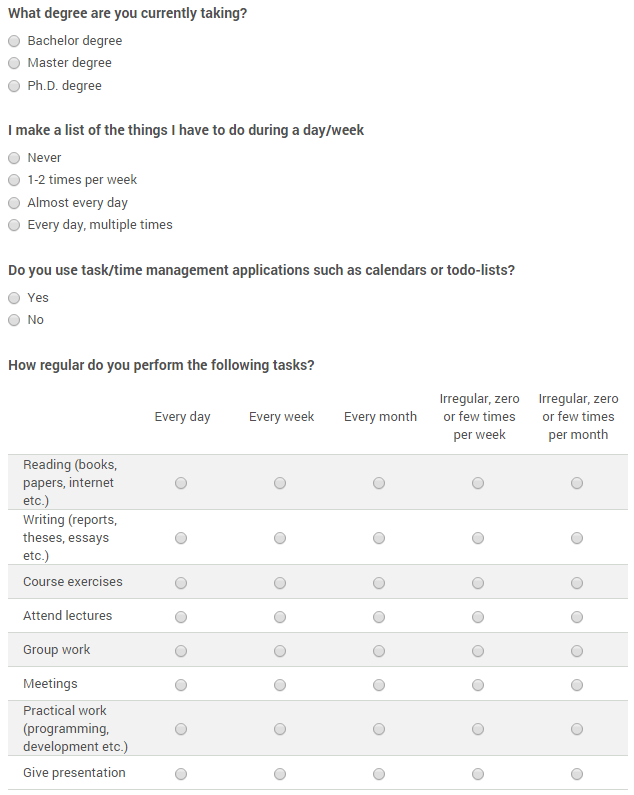
\includegraphics[width=\columnwidth]{appendix/StudentTasks1.PNG}
\caption{}
\label{}
\end{figure}

\begin{figure}[tbp]
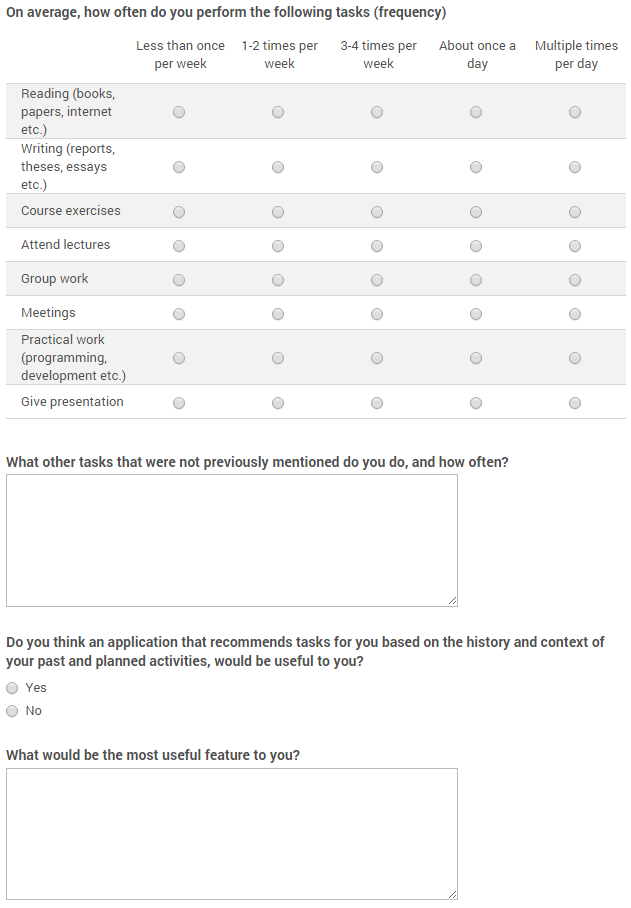
\includegraphics[width=\columnwidth]{appendix/StudentTasks2.PNG}
\caption{}
\label{}
\end{figure}

\end{document}
